\documentclass[paper=a4, fontsize=11pt]{article}

%----------------------------------------------------------------------------------------
%	PACKAGES AND OTHER DOCUMENT CONFIGURATIONS
%----------------------------------------------------------------------------------------

\usepackage{amsmath,amsfonts,amsthm} % Math packages
\usepackage{sectsty} % Allows customizing section commands
\allsectionsfont{\centering \normalfont\scshape} % Make all sections centered, the default font and small caps

\usepackage{fancyhdr} % Custom headers and footers
\pagestyle{fancyplain} % Makes all pages in the document conform to the custom headers and footers
\fancyhead{} % No page header - if you want one, create it in the same way as the footers below
\fancyfoot[L]{} % Empty left footer
\fancyfoot[C]{} % Empty center footer
\fancyfoot[R]{\thepage} % Page numbering for right footer
\renewcommand{\headrulewidth}{0pt} % Remove header underlines
\renewcommand{\footrulewidth}{0pt} % Remove footer underlines
\setlength{\headheight}{13.6pt} % Customize the height of the header

\numberwithin{equation}{section} % Number equations within sections (i.e. 1.1, 1.2, 2.1, 2.2 instead of 1, 2, 3, 4)
\numberwithin{figure}{section} % Number figures within sections (i.e. 1.1, 1.2, 2.1, 2.2 instead of 1, 2, 3, 4)
\numberwithin{table}{section} % Number tables within sections (i.e. 1.1, 1.2, 2.1, 2.2 instead of 1, 2, 3, 4)

%\setlength\parindent{0pt} % Removes all indentation from paragraphs - comment this line for an assignment with lots of text
\setlength{\parskip}{1em}
\renewcommand{\baselinestretch}{1.5}

\usepackage{tikz-qtree}
\usepackage{lscape}

\usepackage{graphicx}
\graphicspath{ {images/} }

\usepackage{xepersian}
\settextfont[Path=fonts/]{Vazir.ttf}
%\setlatintextfont{Times New Roman}

%----------------------------------------------------------------------------------------
%	TITLE SECTION
%----------------------------------------------------------------------------------------

\newcommand{\horrule}[1]{\rule{\linewidth}{#1}} % Create horizontal rule command with 1 argument of height

\title{
\normalfont\normalsize
\includegraphics[scale=0.1]{aut}
\hspace{5cm}
\includegraphics[scale=0.1]{ceit} \\
\textsc دانشگاه صنعتی امیرکبیر \\
\textsc دانشکده مهندسی کامپیوتر و فناوری اطلاعات
\horrule{0.5pt} \\ [0.4cm] % Thin top horizontal rule
\huge معماری سوئیچ و روترهای با کارآیی بالا \\ % The assignment title
\huge تمرین اول \\ % The assignment title
\horrule{2pt} \\ [0.5cm] % Thick bottom horizontal rule
}

\author{پرهام الوانی}

\date{\normalsize\today} % Today's date or a custom date

\begin{document}

\maketitle % Print the title

\section{سوال اول}
\par
در این سوال فرض می‌کنیم عناصر یکسان هستند و تفاوتی با یکدیگر ندارند.

\par
هر عنصر می‌تواند در هر یک از ۱۰۰۰۰ بلوک موجود قرار بگیرد.
فرض می‌کنیم یکی از ۱۰۰۰۰ بلوک خالی باشد، به این ترتیب هر عنصر ۹۹۹۹ انتخاب خواهد داشت.
باید به این تکته توجه داشت که برای جلوگیری از شمارش جندباره‌ی حالت‌ها نیاز است که
مطمئن شویم سایر خانه‌های حداکثر یک عنصر خواهند داشت.
بنابراین احتمال خالی بودن یکی از بلوک‌ها به شرح زیر است:

\begin{align}
\begin{split}
    \frac{\binom{10^4}{1} * \binom{5000 - 1}{10^4 - 2}}{\binom{5000 + 10^4 - 1}{10^4 - 1}}
\end{split}
\end{align}

\par
همانطور که مشخص حاصل رابطه‌ی بالا برابر صفر است زیرا
امکان ندارد بتوان با ۵۰۰۰ عنصر ۱۰۰۰۰ خانه را طوری پر کرد
که دقیقا یک خانه خالی باشد.

\par
اگر فرض کنیم متغیر تصادفی x نشان‌دهنده‌ی تعداد بلوک‌های خالی باشد،
امید ریاضی x متوسط تعداد بلوک‌های خالی خواهد بود
به این ترتیب داریم:

\begin{align}
\begin{split}
    E[x] = \sum_{n = 0}^{10^4}n\frac{\binom{10^4}{n} * \binom{5000 - 1}{10^4 - n - 1}}{\binom{5000 + 10^4 - 1}{10^4 - 1}}
\end{split}
\end{align}

\par
ابتدا دو عنصر را انتخاب کرده و در یک بلوک مشخص قرار می‌دهیم و سایر عناصر ۹۹۹۹ انتخاب خواهند داشت.
اگر فرض کنیم که بلوک دو عنصری از پیش مشخص شده است خواهیم داشت:

\begin{align}
\begin{split}
    \frac{\binom{5000 - 1 + 10^4 - 1}{10^4 - 1}}{\binom{5000 + 10^4 - 1}{10^4 - 1}}
\end{split}
\end{align}

\par
اگر فرض کنیم متغیر تصادفی y نشان‌دهنده‌ی تعداد بلوک‌های دو عنصری باشد
متوسط تعداد بلوک‌های دو عنصری امید ریاضی y خواهد بود.
نکته‌ی اصلی در این روش محاسبه‌ی تعداد بلوک‌های دو عنصری بدون چندباره شماری است،
برای این منظور می‌بایست مطمئن شویم که سایر بلوک‌ها دو عنصری نخواهند بود، یعنی
صفر، یک یا بیش از دو عنصر دارند.

\section{سوال دوم}
\par
برای جستجو در اولین گام بلوک مورد نظر مشخص می‌شود و سپس جستجو در همان بلوک صورت می‌پذیرد.
از آنجایی که جستجو در بلوک صورت می‌پذیرد پس زمان آن به اندازه‌ی بلوک وابسته است،
اندازه‌ی هر بلوک در صورتی که تعداد عناصر آن‌ها با یکدیگر برابر باشد
$n/m$
می‌باشد.

$$
search = O(n/m)
$$

\par
حافظه‌ی مصرفی این روش اگر تعداد عناصر همه‌ی بلوک‌ها با یکدیگر برابر باشد
به اندازه‌ی عناصر موجود خواهد بود ولی
در صورتی که این امر اتفاق نیافتد
حافظه‌ی مصرفی این روش از تعداد عناصر موجود بیشتر خواهد بود.

$$
memroy = \Omega(n/m)
$$

\par
برای به روزرسانی تنها نیاز است که بلوک موردنظر پیدا شود
و در ادامه محتوای آن به روزرسانی شود
بنابراین زمان اجرای به روزرسانی با جستجو تفاوتی ندارد.

\section{سوال سوم}

\begin{landscape}
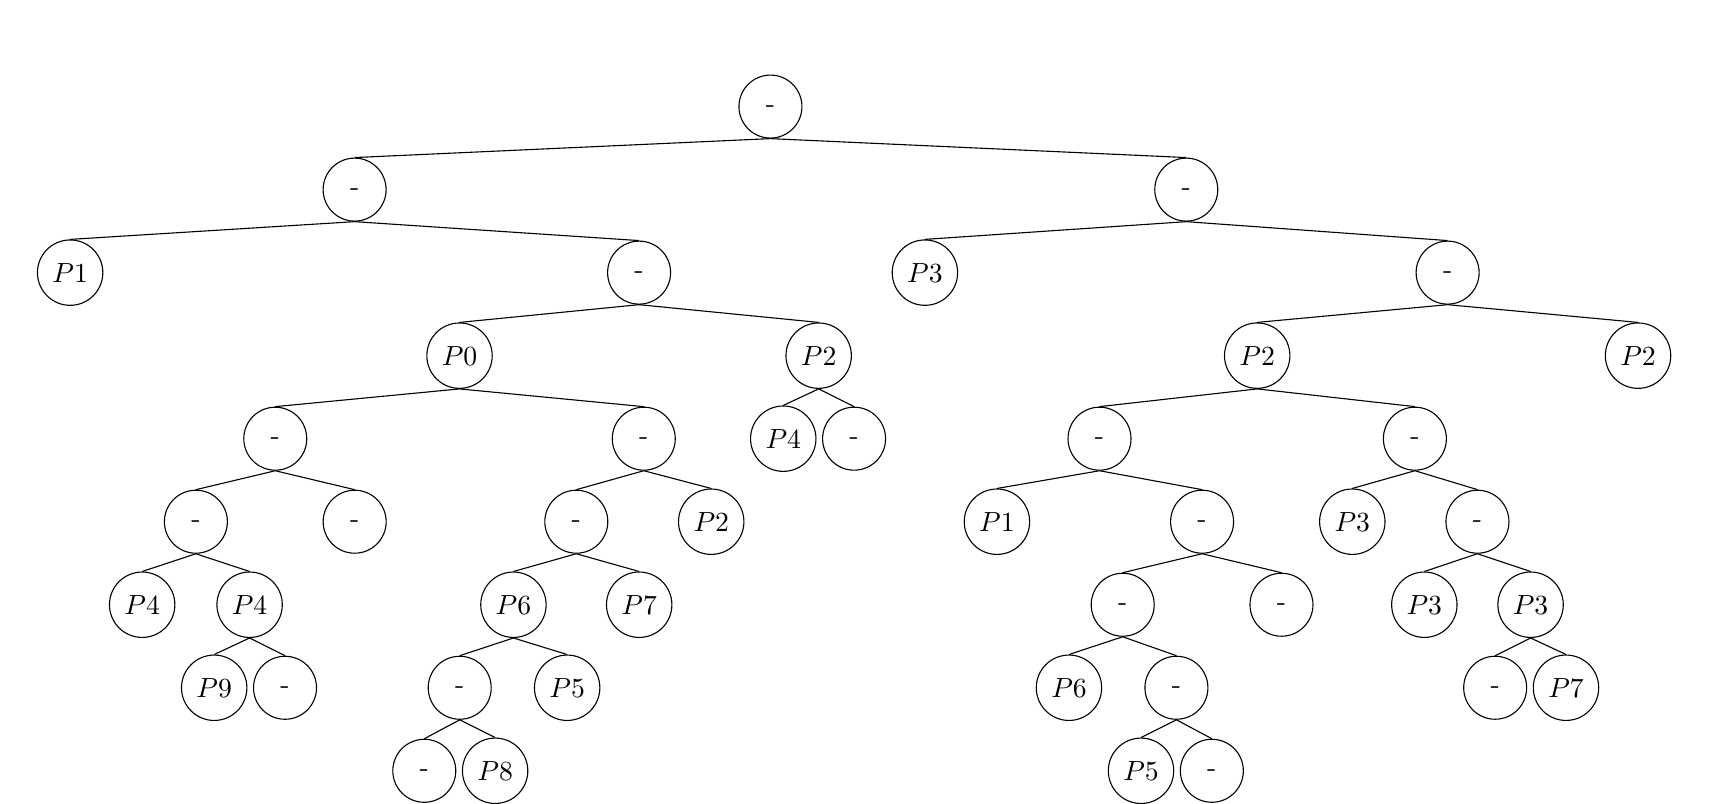
\begin{tikzpicture}[every tree node/.style={draw, circle, minimum width=0.8cm}]
    \matrix{
        \Tree
        [.-
            % 0
            [.- 
                % 00
                [.$P1$ ]
                % 01
                [.- 
                    % 010
                    [.$P0$
                        % 010 0
                        [.-
                            % 010 00
                            [.- $P4$
                                [.$P4$ $P9$ - ]
                            ]
                            % 010 01
                            [.- ]
                        ]
                        % 010 1
                        [.-
                            % 010 10
                            [.- 
                                [.$P6$
                                    [.- - $P8$ ]
                                    [.$P5$ ]
                                ]
                                [.$P7$ ]
                            ]
                            % 010 11
                            [.$P2$ ]
                        ]
                    ]
                    % 011
                    [.$P2$ $P4$ - ]
                ]
            ]
            % 1
            [.-
                % 10
                [.$P3$ ]
                % 11
                [.-
                    % 110
                    [.$P2$
                        % 110 0
                        [.-
                            % 110 00
                            [.$P1$ ]
                            % 110 01
                            [.-
                                % 110 010
                                [.-
                                    [.$P6$ ]
                                    [.- $P5$ - ]
                                ]
                                % 110 011
                                [.- ]
                            ]
                        ]
                        % 110 1
                        [.-
                            % 110 10
                            [.$P3$ ]
                            % 110 11
                            [.-
                                [.$P3$ ]
                                [.$P3$ - $P7$ ]
                            ]
                        ]
                    ]
                    [.$P2$ ]
                ]
            ]
        ]
        &
    \\};
\end{tikzpicture}
\end{landscape}

\section{سوال چهارم}
\par
در ابتدا درخت دودویی که با تعداد \lr{prefix}ها شماره‌گذاری شده است، رسم می‌کنیم.


\begin{center}
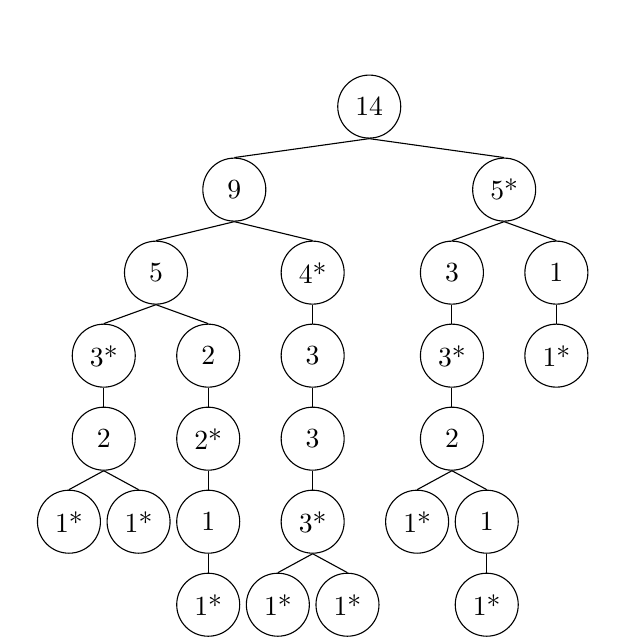
\begin{tikzpicture}[every tree node/.style={draw, circle, minimum width=0.8cm}]
    \matrix{
        \Tree
            [.14
                [.9
                    [.5
                        [.3*
                            [.2 1* 1* ]
                        ]
                        [.2
                            [.2*
                                [.1 1* ]
                            ]
                        ]
                    ]
                    [.4*
                        [.3
                            [.3
                                [.3* 1* 1* ]
                            ]
                        ]
                    ]
                ]
                [.5*
                    [.3
                        [.3*
                            [.2 1*
                                [.1 1* ]
                            ]
                        ]
                    ]
                    [.1 1* ]
                ]
            ]
        &
    \\};
\end{tikzpicture}
\end{center}

\par
روش \lr{subtree-spliting}

\begin{center}
\begin{latin}
\begin{tabular}{ l  c  c  c }
    \hline
    Index & Bucket Prefixes & Bucket Size & Covering Prefix \\
    \hline
    $000^*$ & $000^*, 00010^*, 00011^*$ & 3 & $000^*$ \\
    $00^*$ & $0011^*, 001110^*$ & 2 & --- \\
    $0*$ & $01^*, 01101^*, 011010^0, 011011^*$ & 4 & --- \\
    $10^*$ & $100^*, 10010^*, 100110^*$ & 3 & $1^*$ \\ 
    $*$ & $1^*, 111^*$ & 2 & --- \\
    \hline
\end{tabular}
\end{latin}
\end{center}

\par
ورش \lr{post-order spliting}

\begin{center}
\begin{latin}
\begin{tabular}{ l  c  c  c }
    \hline
    Index & Bucket Prefixes & Bucket Size & Covering Prefix \\
    \hline
    $000^*, 00111^*$ & $000^*, 00010^*, 00011^*, 001110^*$ & 4 & $000^*, 0011^*$ \\
    $00^*, 011^*$ & $0011^*, 01101^*, 011010^*, 011011^*$ & 4 & $01^*$ \\
    $0^*, 10^*$ & $01^*, 100^*, 10010^*, 100110^*$ & 4 & $1^*$ \\
    $*$ & $1^*, 111^*$ & 2 & --- \\
    \hline
\end{tabular}
\end{latin}
\end{center}

\section{سوال پنجم}
\subsection{}
\par
امروزه با افزایش داده‌ها در دیتاسنترها نیاز به توان پردازشی بیشتر و ارتباطات داخلی سریعتری است.
استفاده از تکنولوژی‌های الکتریکی برای انتقال داده محدودیت‌های زیادی دارد، مانند دخالت درونی\footnote{inter-symbol interference}.
یک پاسخ طبیعی به این مشکل استفاده از تکنولوژی‌های نوری است، این تکنولوژی‌ها توانایی سوئیچیگ و نرخ ارسال
بالایی دارند.

\par
استفاده از تکنولوژی‌های نوری مصرف انرژی و فضای بیشتری نسبت به تکنولوژی‌های الکتریکی دارد.
مطالعات زیادی برای ریلکس کردن این موارد صورت گرفته است.

\par
این مقاله در نهایت به دنبال یافتن پاسخ برای افزایش نرخ داده‌ها در دیتاسنترها به وسیله‌ی شبکه‌های نوری و
حل مشکلات این نوع شبکه‌ها در دیتاسنترها است.

\subsection{}
\par
در معماری \lr{switch-centric}
تنها ارتباطات سوئیچ-سوئیچ و سرور-سوئیچ وجود دارد و ارتباطات سرور-سرور وجود ندارد
مانند \lr{fat-tree}.

\begin{center}
\includegraphics[scale=0.5]{fat_tree.png}
\end{center}

\par
این روش سرعت پردازش زیادی داشته ولی مصرف توان و هزینه‌ی زیادی دارد.
این روش برنامه‌پذیری کمی دارد.

\par
در معماری \lr{server-centric}
تنها ارتباطات سرور-سرور و سرور-سوئیچ وجود دارد و ارتباطات سوئیچ-سوئیچ وجود ندارد
مانند \lr{BCube}.

\begin{center}
\includegraphics[scale=0.5]{bcube.jpg}
\end{center}

\par
در این معماری تاخیر پردازشی بیشتر از روش \lr{switch-centric}
است ولی قابلیت برنامه‌پذیری بیشتری نسبت به آن روش وجود دارد.

\subsection{}
\begin{enumerate}
\item
بالاترین سطح ترافیک نماینده‌ی ترافیک بین رک‌ها است،
طول لینک در این ارتباطات بین چند متر تا چند صد متر می‌باشد.
\item
ارتباطات درون تجهیز رک می‌توانند طول لینکی بین ۱۵ سانتی‌متر تا چند متر داشته باشند.
\item
ارتباطات بین چیپ‌ها در یک ماژول که طول لینکشان کمتر از ۲۵ سانتی‌متر می‌باشد.
\item
ارتباطات روی چیپ‌ها که طولشان زیر ۲ سانتی‌متر است.
\end{enumerate}
\par
ارتباطات در ابعاد مختلف مس‌توانند از معماری‌ها و تکنولوژی‌های مختلفی استفاده کنند
زیرا پارامترها و اهداف طراحی آن‌ها با یکدیگر متفاوت است.

\subsection{}
\par
مشکل مهمی که مقیاس‌پذیری و مدیریت سیستم‌های مقیاس-بزرگ را محدود می‌کند تعداد زیاد لینک‌های لازم برای ارتباطات داخلی است
که باعث تعداد زیاد کابل‌ها می‌گردد.
این مشکل عموما به عنوان
\lr{wiriing problem}
شناخته می‌شود.

\par
روش \lr{2D Torus} از نظر تعداد لینک‌ها
با توجه به مقایسه‌ای که در مقاله صورت گرفته است مقیاس‌پذیری بیشتری دارد.

\subsection{}
\par
معماری سوئیچیگ \lr{banyan}
یک معماری چند مرحله‌ای است که دارای \lr{blocking}
است.
\par
معماری سوئیچینگ \lr{cantor}
یک معماری چند مرحله‌ای است که دارای \lr{blocking}
نیست.
در این معماری مستقل از اینکه ارتباطات چگونه ساخته می‌شوند شبکه‌ی حاصل جهت سوئیچینگ دارای
\lr{blocking} نخواهد بود.

\end{document}
